% !TeX root = ../comp_methods_main.tex
%==========================================================
%=========================================================
\chapter{Machine Learning}
%=========================================================
%=========================================================


%-----------------------------------------------------------------------
%======================================================================
\section{Basics of machine learning}
%========================================================================
%--------------------------------------------------------


%=================================================================
\subsection{Learning paradigmes}
%=================================================================

We have the following
\begin{itemize}
    \item \textbf{Supervised learning}. This can be done even without machine learning e.g using regression techniques or some polynomial fitting. After the model has been trained on a labelled dataset, it can be used to predict labels for new data. Examples include classification tasks (e.g., identifying particles as electrons or muons) and regression tasks (e.g., predicting energy levels).
    \item \textbf{Unsupervised learning}. The data does not come with labels. That is we have data but we do not really know what they `mean'. Think of clustering of objects: for example jet clustering algorithms or flavor tagging. The goal is to find and highlight structures in the data.
    \item \textbf{Reinforcement learning}. It is one of the most recent methods. The model learns by interacting with an environment and receiving feedback in the form of rewards or penalties. It allows for real-time decisions. The easiest example is game playing e.g. training an agent to play chess or a videogame. Look at this video of google deep mind learning how to play Atari games: \url{https://youtu.be/V1eYniJ0Rnk?si=0pD-iUJoDWCsZw5h}.
    In the context of HEP..
\end{itemize}
Of course all of this comes with an inane amount of algorithms and techniques, and there is no golden standard that works for everything. The choice of algorithm depends on the specific problem, the nature of the data, and the desired outcomes.


%-------------------------------------------------------------------
\subsection{Supervised learning algorithms}
%-------------------------------------------------------------------


\begin{mytheorem}[Linear regression \& generalized linear models]
Linear regression is a fundamental algorithm used in supervised learning for predicting a continuous target variable based on one or more input features. The goal of linear regression is to find the best-fitting linear relationship between the input features and the target variable.

Namely given some data points \((x_1, y_1), (x_2, y_2), \ldots, (x_n, y_n)\), where \(x_i\in \R^s\) represents the input features and \(y_i\in \R^t\) represents the corresponding target variable, linear regression aims to find a linear function of the form:
\begin{align}
    \hat{y}(x) = W x + b
\end{align}
Then we choose the matrix and the bias so as to minimeze the cost function, typically the mean squared error (MSE):
\begin{align}\label{eq:mse}
    J(W, b) = \frac{1}{n} \sum_{i=1}^{n} \left\| y_i - \hat{y}(x_i) \right\|^2
\end{align}
The solution can be found using various optimization techniques, such as gradient descent or closed-form solutions (e.g., normal equations).

Generalized linear models (GLMs) extend linear regression to handle a wider range of data types and distributions. GLMs consist of three components:
\begin{itemize}
    \item A linear predictor: \( \eta = W x + b \)
    \item A link function: \( g(\mu) = \eta \), which relates the mean of the target variable \( \mu \) to the linear predictor \( \eta \).
    \item A probability distribution from the exponential family (e.g., normal, binomial, Poisson) that describes the distribution of the target variable.
\end{itemize}
%
\end{mytheorem}


Of course there is a \textbf{tradeoff} between \textbf{model complexity vs interpretability}. Linear regression is simple and interpretable but may not capture complex relationships, while more complex models (e.g. neural networks) can capture intricate patterns but may be harder to interpret.

\begin{figure}[h]
\centering
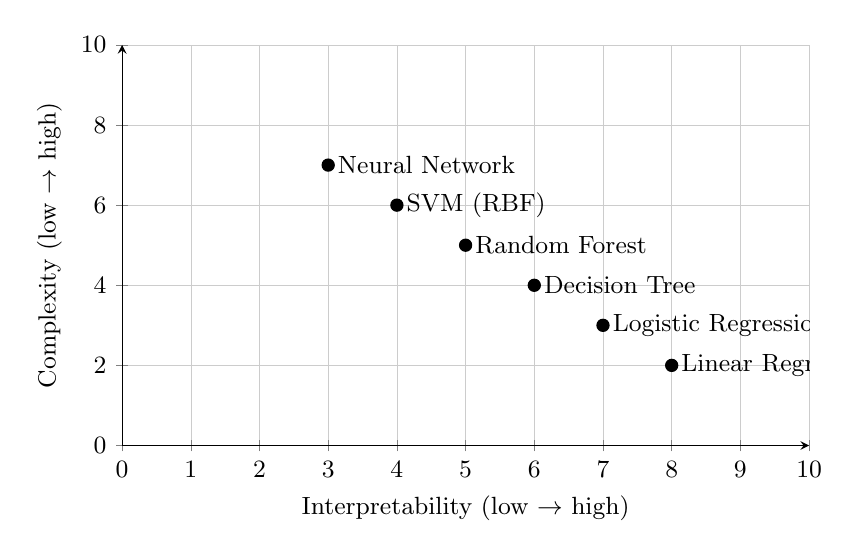
\begin{tikzpicture}
\begin{axis}[
    width=0.85\linewidth,
    height=0.55\linewidth,
    xlabel={Interpretability (low $\rightarrow$ high)},
    ylabel={Complexity (low $\rightarrow$ high)},
    xmin=0, xmax=10,
    ymin=0, ymax=10,
    grid=both,
    major grid style={line width=0.2pt, draw=gray!40},
    minor grid style={line width=0.1pt, draw=gray!20},
    tick label style={font=\small},
    label style={font=\small},
    axis lines=left,
]

\addplot[
    only marks,
    mark=*,
    mark size=2.2pt,
    color=black
] coordinates {
    (8,2) [Linear Regression]
    (7,3) [Logistic Regression]
    (6,4) [Decision Tree]
    (5,5) [Random Forest]
    (4,6) [SVM (RBF)]
    (3,7) [Neural Network]
};

\node[anchor=west, font=\small] at (axis cs:8,2) {Linear Regression};
\node[anchor=west, font=\small] at (axis cs:7,3) {Logistic Regression};
\node[anchor=west, font=\small] at (axis cs:6,4) {Decision Tree};
\node[anchor=west, font=\small] at (axis cs:5,5) {Random Forest};
\node[anchor=west, font=\small] at (axis cs:4,6) {SVM (RBF)};
\node[anchor=west, font=\small] at (axis cs:3,7) {Neural Network};

\end{axis}
\end{tikzpicture}
\caption{Interpretability vs. complexity of common methods.}
\end{figure}


The second \textbf{tradeoff} is between \textbf{underfitting} vs \textbf{overfitting}. 
Your model should be complex enough to capture the underlying patterns in the data (avoiding underfitting), but not so complex that it captures noise or random fluctuations (avoiding overfitting). Techniques such as cross-validation, regularization, and early stopping can help manage this tradeoff.


\begin{mytheorem}[Assessing the performance of supervised learning models]
To evaluate the performance of supervised learning models, we can use various metrics depending on whether the task is regression or classification.
For regression tasks, common metrics include: cost/loss functions, Mean Squared Error (MSE) \eqref{eq:mse}, Root Mean Squared Error (RMSE), Mean Absolute Error (MAE), and R-squared (\(R^2\)).
For classification tasks, common metrics include: accuracy, precision, recall, F1-score, and Area Under the Receiver Operating Characteristic Curve (AUC-ROC curve).
%

If data are correlated, we can include some correlation matrix $\sigma$ in the cost function, e.g. for MSE we would have
\begin{align}
    J(W, b) = \frac{1}{n} \sum_{i=1}^{n} \left( y_i - \hat{y}(x_i) \right)^T \sigma^{-1} \left( y_i - \hat{y}(x_i) \right)
\end{align}
where the covariance matrix $\sigma$ encodes the correlations between different data points and is typically estimated from the training data.

Yet another method for linear regression if the negative log-likelihood. Assuming the errors are normally distributed with mean zero and variance \(\sigma^2\), the negative log-likelihood can be expressed as:
\begin{align}
    J = \frac{1}{2\sigma^2} \sum_{i=1}^{n} \left( y_i - \hat{y}(x_i) \right)^2 + \frac{n}{2} \log(2\pi\sigma^2)
\end{align}
Minimizing this negative log-likelihood is equivalent to minimizing the MSE, but it provides a probabilistic interpretation of the model.

Another method for binary classification is cross-entropy loss. Given true labels \(y_i\) (0 or 1) and predicted probabilities \(\hat{y}(x_i)\), the cross-entropy loss is defined as:
\begin{align}
    J = -\frac{1}{n} \sum_{i=1}^{n} \left[ y_i \log(\hat{y}(x_i)) + (1 - y_i) \log(1 - \hat{y}(x_i)) \right]
\end{align}
This loss function penalizes incorrect predictions more heavily, especially when the predicted probability is far from the true label.
%
\end{mytheorem}



\begin{mytheorem}[Issues of supervised learning]
There are several problems we sould rather avoid and side aim to achieve.
\begin{itemize}
    \item The model should NOT learn the noise in the training data (overfitting). 
    \item The model should generalize well to unseen data (avoid underfitting).
\end{itemize}
To address these issues, we typically split the dataset into training, validation, and test sets. The training set is used to train the model, the validation set is used to tune hyperparameters and assess model performance during training, and the test set is used to evaluate the final model's performance on unseen data.

The best way to assess the optimal capacity is to stop when capacity is such that the \textbf{bias} and the \textbf{variance} cross each other.
Indeed, overfitting is associated with high variance and low bias, while underfitting is associated with high bias and low variance. The goal is to find a balance between bias and variance that minimizes the overall prediction error (cf. plots).
%

To penalize overfitting we can add weights to the cost function that penalize large coefficients, which would make the model very sensible to small changes in the input.
For example in linear regression we can add a regularization term to the cost function:
\begin{align}
    J(W, b) = \frac{1}{n} \sum_{i=1}^{n} \left\| y_i - \hat{y}(x_i) \right\|^2 + \lambda \|W\|^2
\end{align}
Such a term is called L2 regularization (or Ridge regularization) and helps prevent overfitting by discouraging large weights $W$ in the model. The hyperparameter \(\lambda\) controls the strength of the regularization. A larger \(\lambda\) increases the penalty for large weights, leading to a simpler model, but a huge \(\lambda\) will lead to underfitting!
\end{mytheorem}